\documentclass[border=5pt]{standalone}
\usepackage{tikz}
\usetikzlibrary{shapes,arrows.meta,positioning,backgrounds,fit,calc,decorations.pathreplacing}
\usepackage{amsmath}
\usepackage{xcolor}

% Colours
\definecolor{t1col}{RGB}{66,165,245}   % light blue
\definecolor{t2col}{RGB}{102,187,106}  % green
\definecolor{t3col}{RGB}{239,83,80}    % red
\definecolor{t4col}{RGB}{171,71,188}   % purple
\definecolor{arrcol}{RGB}{120,120,140}
\definecolor{wpblue}{RGB}{66,133,244}
\definecolor{wpred}{RGB}{234,67,53}
\definecolor{wpyellow}{RGB}{200,160,5}

\begin{document}
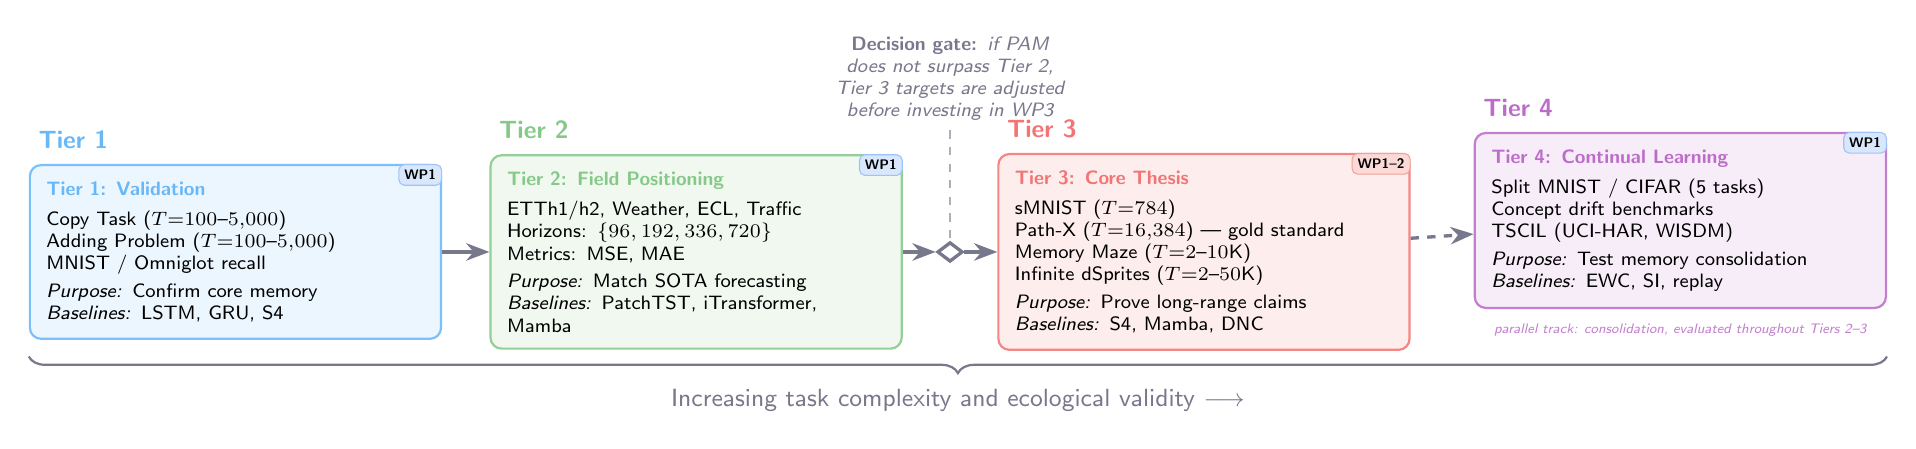
\begin{tikzpicture}[
    >=Stealth,
    tierbox/.style={draw=#1!70, fill=#1!10, rounded corners=4pt, thick,
                    minimum height=1.8cm, text width=4.8cm, align=left,
                    font=\scriptsize\sffamily, inner sep=6pt},
    tierhead/.style={font=\small\sffamily\bfseries, color=#1!80},
    wpbadge/.style={font=\tiny\sffamily\bfseries, rounded corners=2pt,
                    fill=#1!20, draw=#1!50, inner sep=2pt},
    arr/.style={->, very thick, color=arrcol},
    node distance=0.5cm,
]

% ============ TIER 1 ============
\node[tierbox=t1col] (t1) {
  \textcolor{t1col!80}{\textbf{Tier 1: Validation}}\\[3pt]
  Copy Task ($T{=}100$--$5{,}000$)\\
  Adding Problem ($T{=}100$--$5{,}000$)\\
  MNIST / Omniglot recall\\[2pt]
  \textit{Purpose:} Confirm core memory\\
  \textit{Baselines:} LSTM, GRU, S4
};
\node[wpbadge=wpblue, anchor=north east] at (t1.north east) {WP1};
\node[tierhead=t1col, anchor=south west] at (t1.north west) [yshift=2pt] {Tier 1};

% ============ TIER 2 ============
\node[tierbox=t2col, right=0.6cm of t1] (t2) {
  \textcolor{t2col!80}{\textbf{Tier 2: Field Positioning}}\\[3pt]
  ETTh1/h2, Weather, ECL, Traffic\\
  Horizons: $\{96, 192, 336, 720\}$\\
  Metrics: MSE, MAE\\[2pt]
  \textit{Purpose:} Match SOTA forecasting\\
  \textit{Baselines:} PatchTST, iTransformer, Mamba
};
\node[wpbadge=wpblue, anchor=north east] at (t2.north east) {WP1};
\node[tierhead=t2col, anchor=south west] at (t2.north west) [yshift=2pt] {Tier 2};

% ============ TIER 3 ============
\node[tierbox=t3col, right=1.2cm of t2] (t3) {
  \textcolor{t3col!80}{\textbf{Tier 3: Core Thesis}}\\[3pt]
  sMNIST ($T{=}784$)\\
  Path-X ($T{=}16{,}384$) --- gold standard\\
  Memory Maze ($T{=}2$--$10$K)\\
  Infinite dSprites ($T{=}2$--$50$K)\\[2pt]
  \textit{Purpose:} Prove long-range claims\\
  \textit{Baselines:} S4, Mamba, DNC
};
\node[wpbadge=wpred, anchor=north east] at (t3.north east) {WP1--2};
\node[tierhead=t3col, anchor=south west] at (t3.north west) [yshift=2pt] {Tier 3};

% ============ TIER 4 (parallel consolidation track) ============
\node[tierbox=t4col, right=0.8cm of t3, yshift=0.4cm] (t4) {
  \textcolor{t4col!80}{\textbf{Tier 4: Continual Learning}}\\[3pt]
  Split MNIST / CIFAR (5 tasks)\\
  Concept drift benchmarks\\
  TSCIL (UCI-HAR, WISDM)\\[2pt]
  \textit{Purpose:} Test memory consolidation\\
  \textit{Baselines:} EWC, SI, replay
};
\node[wpbadge=wpblue, anchor=north east] at (t4.north east) {WP1};
\node[tierhead=t4col, anchor=south west] at (t4.north west) [yshift=2pt] {Tier 4};

% ============ PROGRESSION ARROWS + DECISION GATE ============
\draw[arr] (t1) -- (t2);

% gate diamond ON the Tier 2 -> Tier 3 arrow
\node[diamond, draw=arrcol, fill=white, very thick, inner sep=2pt, aspect=1.3]
  (gate) at ($(t2.east)!0.5!(t3.west)$) {};
\draw[arr] (t2) -- (gate);
\draw[arr] (gate) -- (t3);

\node[font=\scriptsize\sffamily\itshape, color=arrcol, text width=4.8cm, align=center]
  (gatetext) at ($(gate)+(0,2.2)$) {
  \textbf{Decision gate:} if PAM does not surpass Tier~2,\\Tier~3 targets are adjusted before investing in WP3
};
\draw[dashed, thin, arrcol!60] (gatetext.south) -- (gate.north);

% Tier 4 runs alongside Tiers 2--3, not after them
\draw[arr, dashed] (t3) -- (t4);
\node[font=\tiny\sffamily\itshape, color=t4col!70, anchor=north] at (t4.south) [yshift=-2pt]
  {parallel track: consolidation, evaluated throughout Tiers 2--3};

% ============ BOTTOM: Progression label ============
\draw[decorate, decoration={brace, amplitude=6pt, mirror, raise=6pt}, thick, color=arrcol]
  (t1.south west) -- (t4.south east |- t1.south)
  node[midway, below=14pt, font=\small\sffamily, color=arrcol] {
    Increasing task complexity and ecological validity $\longrightarrow$
  };

\end{tikzpicture}
\end{document}
